\documentclass[11pt,a4paper]{article}

% ─────────────────────────────────────────────────────────────
%  Human Health and Environment — Data Science Laboratory
%  Written report (max 4 pages + max 2 appendix pages)
%  Font 10–12 pt, single line spacing  ✔ (11pt, default \singlespacing)
% ─────────────────────────────────────────────────────────────
\usepackage[utf8]{inputenc}
\usepackage[T1]{fontenc}
\usepackage[english]{babel}
\usepackage[a4paper,margin=2.1cm]{geometry}
\usepackage{graphicx}
\usepackage{amssymb}
\usepackage{booktabs}
\usepackage{caption}
\usepackage{subcaption}
\usepackage{enumitem}
\usepackage{xcolor}
\usepackage{titlesec}
\usepackage[hidelinks]{hyperref}

\graphicspath{{../data/figures/}}

% Compact but readable spacing to respect the 4-page limit
\setlist{nosep,leftmargin=1.3em,topsep=2pt}
\titlespacing*{\section}{0pt}{6pt}{3pt}
\titlespacing*{\subsection}{0pt}{4pt}{2pt}
\titleformat{\section}{\normalfont\large\bfseries\color{black!85}}{\thesection.}{0.5em}{}
\titleformat{\subsection}{\normalfont\normalsize\bfseries\color{black!70}}{\thesubsection}{0.5em}{}
\setlength{\parskip}{2pt}
\setlength{\parindent}{0pt}
\captionsetup{font=small,labelfont=bf}

\title{\vspace{-1.4cm}\textbf{Marine Litter Hazard Assessment in the Sardinian Sea}\\[2pt]
\large A multi-compartment spatial hazard index from ISPRA monitoring data (2018--2023)}
\author{Daniele Uras \quad\textbar\quad Filippo Saccomano\\[2pt]
\normalsize Human Health and Environment --- Data Science Laboratory, Politecnico di Milano}
\date{\normalsize \today}

\begin{document}
\maketitle
\vspace{-0.7cm}

% ═══════════════════════════════════════════════════════════════
\section{Introduction and objective}
The Mediterranean concentrates roughly 7\% of the world's floating marine plastic on less than
1\% of the global ocean surface. Sardinia couples a 1{,}849~km coastline with intense seasonal
tourism and sensitive habitats (\textit{Posidonia} meadows, coralligenous reefs, \textit{Caretta
caretta}). ISPRA collects marine-litter monitoring data under the EU Marine Strategy Framework
Directive (MSFD, Descriptor~10), but these data had never been \emph{integrated across
compartments} nor analysed spatially at sub-regional scale.

\textbf{Research question.} \textit{How is marine-litter hazard distributed along the Sardinian
coast, and what temporal and statistical patterns emerge from ISPRA data (2018--2023)?} Our answer
is an open, reproducible pipeline that processes eight monitored data compartments and combines the
four most directly hazard-relevant of them into a single spatial \emph{hazard index}, whose
structure is then tested with formal autocorrelation statistics. The remaining compartments are
analysed as pressure context or standalone exploratory layers (Sec.~3). The
deliverable is threefold: a documented code repository, an interactive dashboard, and this report.
Detailed numerical results are deliberately kept brief here and are the focus of the oral
presentation.

\textbf{Data and tools.} Inputs are the ISPRA MSFD modules (beach litter --- \textit{Modulo~4};
floating litter --- \textit{Modulo~2-bis}; microplastics --- \textit{Modulo~2}; D10 turtle-stranding
records for entanglement and ingestion), complemented by CMEMS current reanalysis and ISTAT
tourism statistics. The stack is intentionally minimal and free: Python (\texttt{pandas},
\texttt{numpy}, \texttt{scipy}, \texttt{shapely}, \texttt{matplotlib}) for the analysis, and
React\,+\,Leaflet for the dashboard. Spatial statistics are implemented from first principles
rather than pulled from heavy geostatistics libraries, keeping the environment small and the
methods auditable.

% ═══════════════════════════════════════════════════════════════
\section{Work organisation}
The project was carried out by a two-person team. We worked on a shared GitHub repository
(\texttt{daniele22-u/hhe-labsardinia}) using feature branches and frequent, descriptive commits, so
that every analytical decision is traceable in the version history. Tasks were split by area of
ownership but reviewed jointly; pair work was reserved for the decisions that shape the whole
output (compartment weights, grid resolution, validation strategy). Asynchronous coordination was
handled through the commit log and issue notes rather than scattered files, which kept a single,
linear project narrative.

\begin{table}[h]
\centering
\small
\begin{tabular}{@{}p{2.6cm}p{5.2cm}p{5.2cm}@{}}
\toprule
\textbf{Area} & \textbf{Daniele Uras} & \textbf{Filippo Saccomano}\\
\midrule
Lead & Data engineering, ISPRA retrieval, dashboard & Spatial methods, statistics, EDA\\
Tasks & Module download/filtering, schema harmonisation, React dashboard, repo maintenance &
IDW interpolation, composite index, Moran/LISA/GI*, figures\\
Shared & \multicolumn{2}{l}{Project design, weight choices, validation, report \& presentation}\\
\bottomrule
\end{tabular}
\caption{Division of labour. Ownership is indicative; design choices were made jointly.}
\end{table}

\textbf{Workflow discipline.} A single canonical artefact, \texttt{data/dashboard\_data.json}, is
produced by the pipeline and consumed by every downstream component (figures, dashboard, report).
This ``one source of truth'' avoided drift between team members and made results reproducible: any
member could regenerate the whole output from raw ISPRA files with one command sequence. The same
contract removed a classic two-person failure mode --- divergent intermediate CSVs --- because the
JSON schema is the only interface the two work-streams share. Adding a compartment therefore means
appending one key to the JSON, not renegotiating the whole codebase.

% ═══════════════════════════════════════════════════════════════
\section{Project choices and rationale}
Choices were driven by relevance and reproducibility rather than convenience.

\begin{itemize}
\item \textbf{Scope (MSFD D10, Sardinia).} D10 is the litter descriptor and the only one with
multi-year, multi-compartment Sardinian coverage. Sardinia maximises the pressure/sensitivity
contrast (tourism vs.\ protected habitats), making it a meaningful policy case.

\item \textbf{Many compartments, a deliberate subset in the index.} Beach litter alone is the
standard proxy, but it ignores the physical transport and ecological harm that turn litter into
\emph{hazard}. We therefore collected and analysed eight compartments, then made an explicit choice
about which feed the headline index. \textbf{In the index:} beach and floating litter (the spatial
litter signal), the plastic share of beach material, sea currents (transport), and biological
impact. \textbf{Deliberately excluded from the index} --- each for a specific, defensible reason:
\begin{itemize}
\item \textit{Tourism} is a \emph{driver}, not a hazard state: an index must measure how hazardous
a location \emph{is}, not what causes it. Folding a cause into the effect is a category error, and
since tourism correlates \emph{negatively} with litter ($r\!\approx\!-0.44$) it would perversely
lower the score where pressure is highest. It is far more useful as an independent explanatory
variable (Sec.~6, COVID experiment).
\item \textit{Microplastics} is a legitimate hazard state but has uneven trawl coverage and stops
at 2022 (no 2023 module). Including it would break the cross-year comparability that the global
normalisation is built to guarantee; we keep it as a standalone exploratory layer and flag it as
the prime candidate for future inclusion (Sec.~8).
\item \textit{Seafloor litter} is, for Sardinia, a \emph{synthetic} placeholder (no ISPRA module
released; Sec.~7). Injecting fabricated values into the headline number would be scientifically
indefensible, so it is excluded on principle.
\end{itemize}
Excluding these is not an omission but a guard: adding driver-type, non-comparable or synthetic
signals would weaken, not strengthen, the index. The dashboard still exposes all eight as
toggleable layers, so nothing is hidden --- only the \emph{scored} index is kept clean.

\item \textbf{Composite hazard index (IPCC framing).} The selected compartments are min--max
normalised (globally, for cross-year comparability), interpolated by Inverse Distance Weighting onto
a common 0.12$^{\circ}$ ($\sim$12~km) grid, then combined as a weighted mean: beach\,+\,floating
litter~35\%, plastic share~25\%, currents~20\%, biological impact~20\%. Weights are an explicit,
documented default --- not a fitted black box --- so reviewers can challenge or adjust them live in
the dashboard.

\item \textbf{Spatial statistics (LEC12).} A visual hotspot is not evidence. We added Global
Moran's~I, Local Moran's~I (LISA) and Getis--Ord~GI* to \emph{test} whether clustering is real,
\emph{locate} it, and \emph{grade} its intensity. These were implemented from scratch in NumPy to
keep the environment lightweight and the maths inspectable.

\item \textbf{COVID-19 as a natural experiment.} The 2020 tourism collapse, against an
approximately constant current field, lets us separate human-driven from transport-driven litter ---
a design choice that turns a confounder into evidence.

\item \textbf{Interactive dashboard.} A React/Leaflet dashboard was chosen over static plots so
that non-technical stakeholders (managers, policy makers) can explore years, layers and weights
themselves.
\end{itemize}

% ═══════════════════════════════════════════════════════════════
\section{Workflow completeness and usability}
The pipeline was built to map one-to-one onto the development phases presented in the lectures,
rather than as an ad-hoc script collection. Table~\ref{tab:phases} makes that mapping explicit.

\begin{table}[h]
\centering\small
\begin{tabular}{@{}p{3.2cm}p{5.0cm}p{5.0cm}@{}}
\toprule
\textbf{Lecture phase} & \textbf{What we did} & \textbf{Artefact}\\
\midrule
Data acquisition & ISPRA module retrieval, regional bounding-box filtering, provenance headers &
\texttt{Labenv/}, script headers\\
Cleaning \& harmonisation & Schema unification across years, fixed protocol, coordinate back-fill &
\texttt{01\_data\_cleaning}, \texttt{clean\_all.py}\\
Exploratory analysis & Trends, composition, seasonality, cross-compartment correlations &
\texttt{02\_eda}, figures\\
Modelling & IDW grid, composite index, coastal-segment aggregation, spatial statistics &
\texttt{03\_spatial\_hazard}, \texttt{analysis\_04--10}\\
Integration & Single canonical dataset assembled from all compartments &
\texttt{update\_dashboard\_data.py} $\rightarrow$ JSON\\
Communication & Interactive dashboard, static figures, report, presentation &
\texttt{dashboard-react/}, \texttt{build\_deck.js}\\
\bottomrule
\end{tabular}
\caption{Mapping of the lecture development phases onto concrete project artefacts. Each phase has
an owned, reproducible step rather than being skipped or merged.}
\label{tab:phases}
\end{table}

\textbf{Usability.} Reproducibility on a new machine was treated as a first-class requirement. The
repository ships a README documenting environment setup and a fixed run order (notebooks
\texttt{01}$\rightarrow$\texttt{03}, then scripts \texttt{04}$\rightarrow$\texttt{10}, then
\texttt{update\_dashboard\_data.py}); all paths are relative to the repository root; and every
script header records its data provenance (ISPRA module, bounding box, year range). The dashboard is
a static build served from the generated JSON, so it needs no backend. A clean checkout therefore
regenerates every figure and the full dashboard from the raw files with no manual editing --- the
main usability risk that remains is obtaining the raw ISPRA modules, which require manual download
from the national portal and are documented accordingly.

% ═══════════════════════════════════════════════════════════════
\section{Most relevant results (summary)}
Reported briefly --- detail is reserved for the presentation (figures in Appendix).
\begin{itemize}
\item A persistent \textbf{west-coast hazard corridor} (Alghero--Oristano); the east coast is
consistently low. The gradient appears in every compartment and every year.
\item \textbf{Statistically significant clustering}: Global Moran's~I~$\approx 0.95$
($p<0.001$) for all six years; LISA confirms a coherent High--High hotspot with \emph{zero} spatial
outliers (Appendix, Table~\ref{tab:moran}).
\item \textbf{COVID signal}: mean beach litter fell $\sim$68\% in 2020 with the tourism drop while
currents stayed constant --- evidence of both human and transport drivers --- yet litter did not
return to pre-2020 levels (legacy effect).
\end{itemize}

% ═══════════════════════════════════════════════════════════════
\section{Relevance for policy}
The index is built to be \emph{actionable}. Aggregation to 126 coastal \textit{comuni} converts
abstract grid cells into administrative units, so clean-up budgets and monitoring effort can be
prioritised where hazard is statistically confirmed (the west coast) rather than spread uniformly
along 1{,}849~km of shoreline.

Crucially, both ``positive'' and ``negative'' findings carry policy value. The \emph{positive}
result --- a stable, significant west-coast hotspot --- gives managers a defensible target for
intervention. The \emph{negative} result --- the weak/negative tourism--litter correlation --- is
arguably more informative: it warns that visitor-targeted measures (beach access limits, local
fees) alone will not solve a problem that is partly transport- and legacy-driven, and redirects
attention toward upstream land-based sources and current-aware interception. The COVID natural
experiment sharpens this: litter fell with tourism but did not vanish or rebound to prior levels,
so a credible strategy must combine source reduction with sustained removal of accumulated litter.
Because the dashboard exposes the compartment weights, a decision-maker can stress-test how
robust a priority ranking is to the relative importance assigned to beach, plastic, current and
biological signals.

% ═══════════════════════════════════════════════════════════════
\section{Limitations}
\begin{itemize}
\item Only \textbf{6 beach stations}: sparse support, so IDW smooths aggressively and part of the
very high autocorrelation is inherited from the interpolation, not purely from nature.
\item The \textbf{seafloor compartment is synthetic} (no Sardinian ISPRA seafloor module was
available); it uses real D8 station coordinates as placeholders and is excluded from the headline
index.
\item Scores are \textbf{relative} (min--max within the dataset), not absolute concentrations, so
they compare internally but not against external thresholds.
\item The COVID inference rests on a \textbf{single lockdown year} (low statistical power) and the
pre-COVID mean is inflated by a few extreme surveys (the median change is milder than the mean).
\item Compartments differ in \textbf{sampling effort across years} (e.g.\ floating-litter counts
grow with later, denser campaigns), so cross-year comparisons of raw counts are read cautiously and
the index relies on global normalisation to mitigate this.
\item The composite \textbf{weights are expert-set, not learned}; they are a transparent default
meant to be challenged, and the dashboard lets reviewers test sensitivity, but they are not
optimised against an external hazard ground truth (none exists at this scale).
\end{itemize}

% ═══════════════════════════════════════════════════════════════
\section{Future developments}
Three priorities follow directly from the choices above. \emph{(i)} Promote \textbf{microplastics}
into the scored index once the 2022 coverage gap is closed and the 2023 module is released --- it is
the only excluded compartment that is a genuine hazard state. \emph{(ii)} Replace the synthetic
seafloor layer with real \textbf{MEDITS} trawl data, which would also let it enter the index
honestly. \emph{(iii)} Move from description to explanation with \textbf{spatial regression}
(SAR/SEM, and GWR/MGWR for location-varying drivers) and a \textbf{bi-variate Moran's~I} coupling
beach and floating litter. We would also validate against independent \textbf{citizen-science} beach
clean-ups and publish a per-\textit{comune} policy brief. The modular pipeline and single-JSON
contract make each of these an incremental addition rather than a rewrite.

% ═══════════════════════════════════════════════════════════════
\appendix
\clearpage
\section*{Appendix --- Figures and Tables}
\renewcommand{\thefigure}{A\arabic{figure}}
\renewcommand{\thetable}{A\arabic{table}}
\setcounter{figure}{0}\setcounter{table}{0}

\begin{table}[h]
\centering\small
\begin{tabular}{@{}lcccc@{}}
\toprule
\textbf{Year} & \textbf{Global Moran's I} & \textbf{z} & \textbf{p} & \textbf{Interpretation}\\
\midrule
2018 & 0.965 & 31.4 & 0.000 & clustered\\
2019 & 0.936 & 31.1 & 0.000 & clustered\\
2020 & 0.948 & 32.0 & 0.000 & clustered\\
2021 & 0.943 & 30.0 & 0.000 & clustered\\
2022 & 0.951 & 30.4 & 0.000 & clustered\\
2023 & 0.948 & 30.4 & 0.000 & clustered\\
\bottomrule
\end{tabular}
\caption{Global spatial autocorrelation of the composite hazard index (Queen contiguity,
row-standardised weights, 999-permutation test). Clustering is strong and significant every year.}
\label{tab:moran}
\end{table}

\begin{table}[h]
\centering\small
\begin{tabular}{@{}lccc@{}}
\toprule
\textbf{Metric} & \textbf{Pre-COVID (2018--19)} & \textbf{COVID (2020)} & \textbf{Post (2021--23)}\\
\midrule
Tourist-nights (M/yr)        & 14.3 & 8.7 & 13.4\\
Beach litter (mean items/100\,m) & 830 & 269 & 298\\
Beach litter (median)        & 324 & 176 & 288\\
Current speed (cm/s)         & 13.2 & 12.4 & 11.8\\
Bio events (ENT+ING)         & 44 & 20 & 101\\
\bottomrule
\end{tabular}
\caption{COVID-19 natural experiment. Tourism and beach litter fall together while sea currents
(natural transport driver) stay almost constant.}
\label{tab:covid}
\end{table}

\begin{figure}[h]
\centering
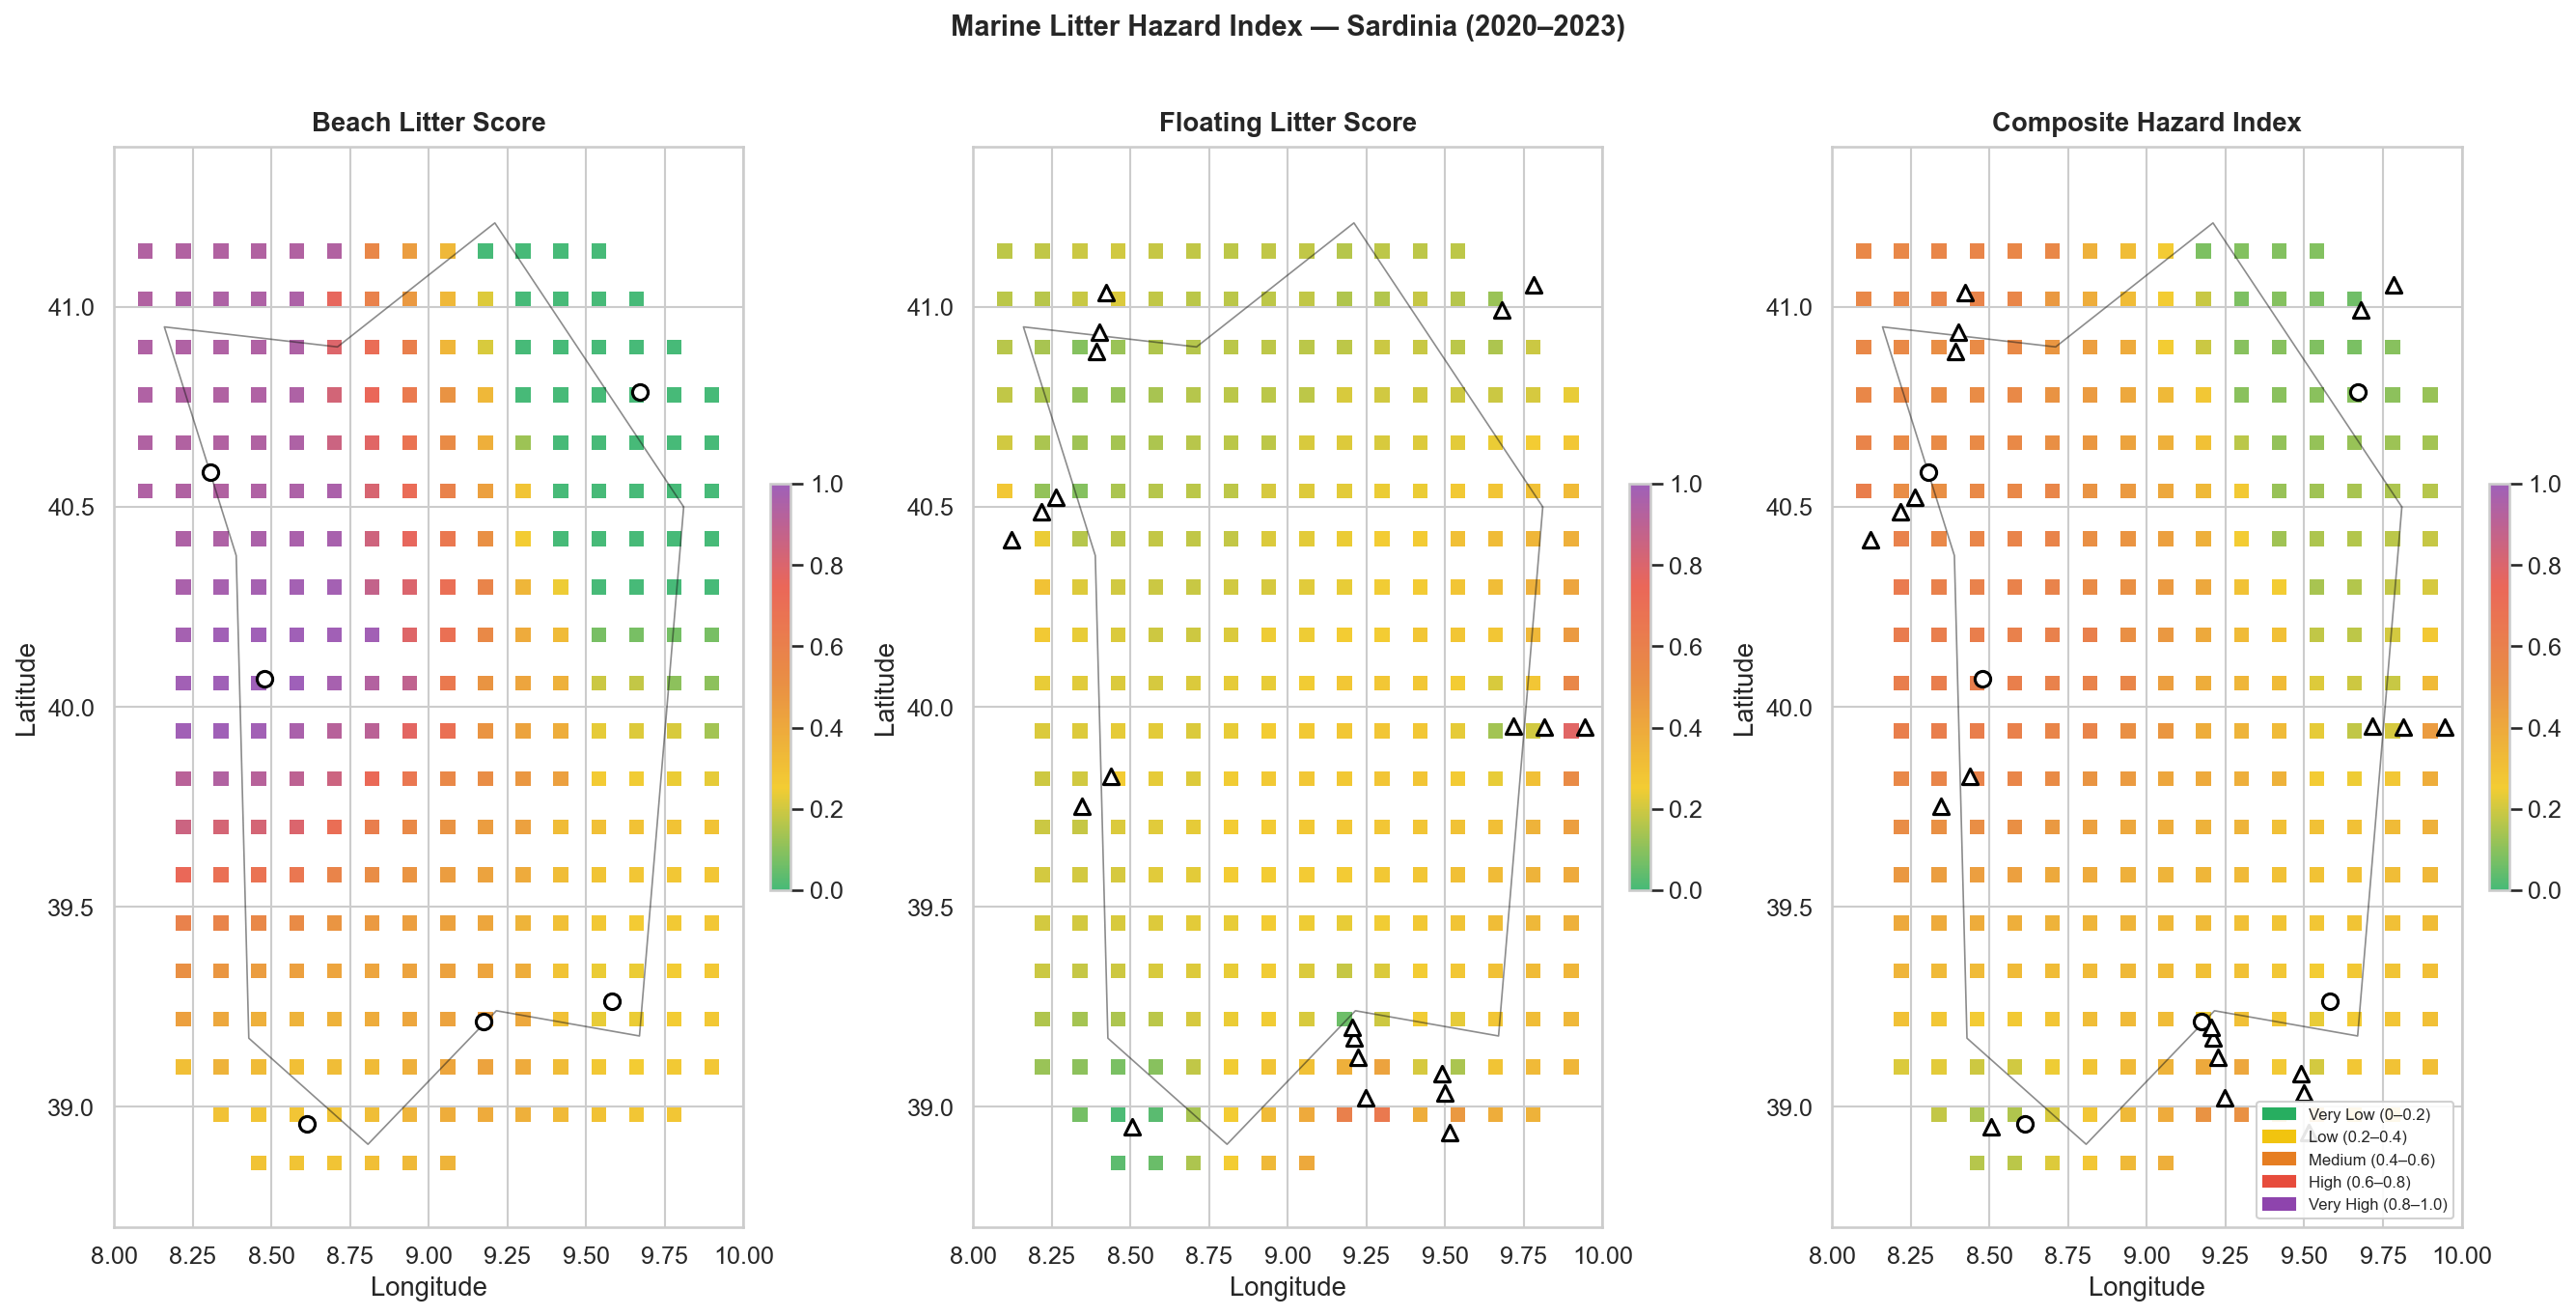
\includegraphics[width=0.93\textwidth]{hazard_index_map.png}
\caption{Composite hazard index --- beach score, floating score and combined index. Markers show
beach ($\bullet$) and offshore ($\blacktriangle$) stations.}
\end{figure}

\begin{figure}[h]
\centering
\begin{subfigure}{0.49\textwidth}\centering
\includegraphics[width=\linewidth]{lisa_cluster_map.png}
\caption{LISA clusters (HH red, LL blue).}\end{subfigure}\hfill
\begin{subfigure}{0.49\textwidth}\centering
\includegraphics[width=\linewidth]{gi_star_map.png}
\caption{Getis--Ord GI* hotspot z-scores.}\end{subfigure}
\caption{Local spatial statistics: a coherent west-coast High--High hotspot, east-coast coldspot,
no spatial outliers.}
\end{figure}

\begin{figure}[h]
\centering
\begin{subfigure}{0.49\textwidth}\centering
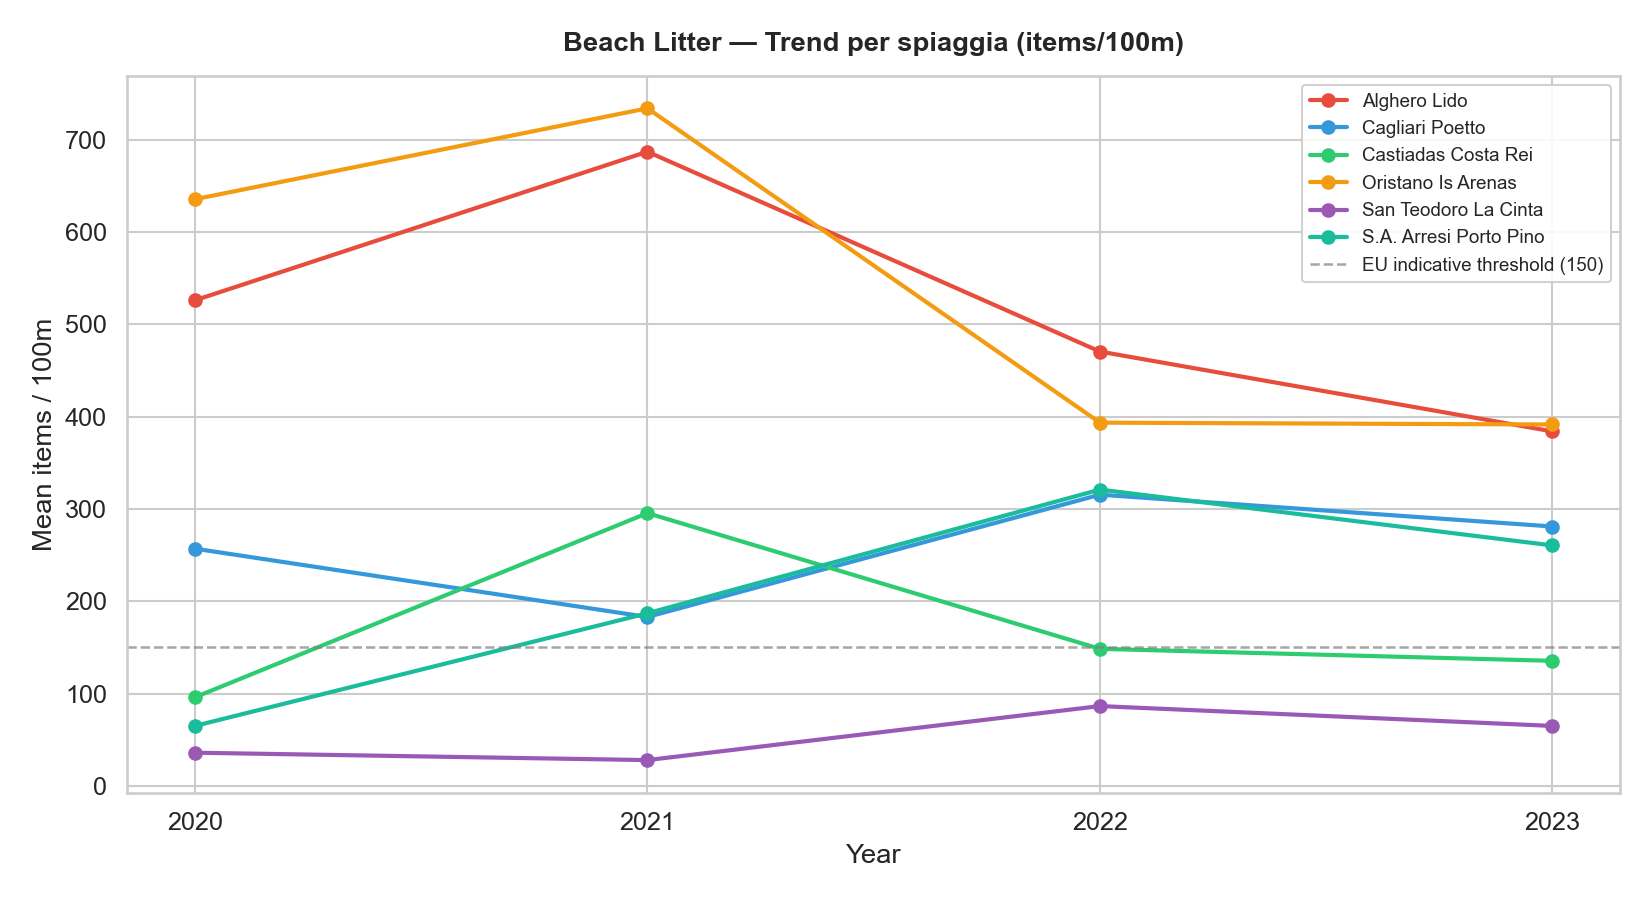
\includegraphics[width=\linewidth]{beach_trend_per_station.png}
\caption{Beach litter trend per station.}\end{subfigure}\hfill
\begin{subfigure}{0.49\textwidth}\centering
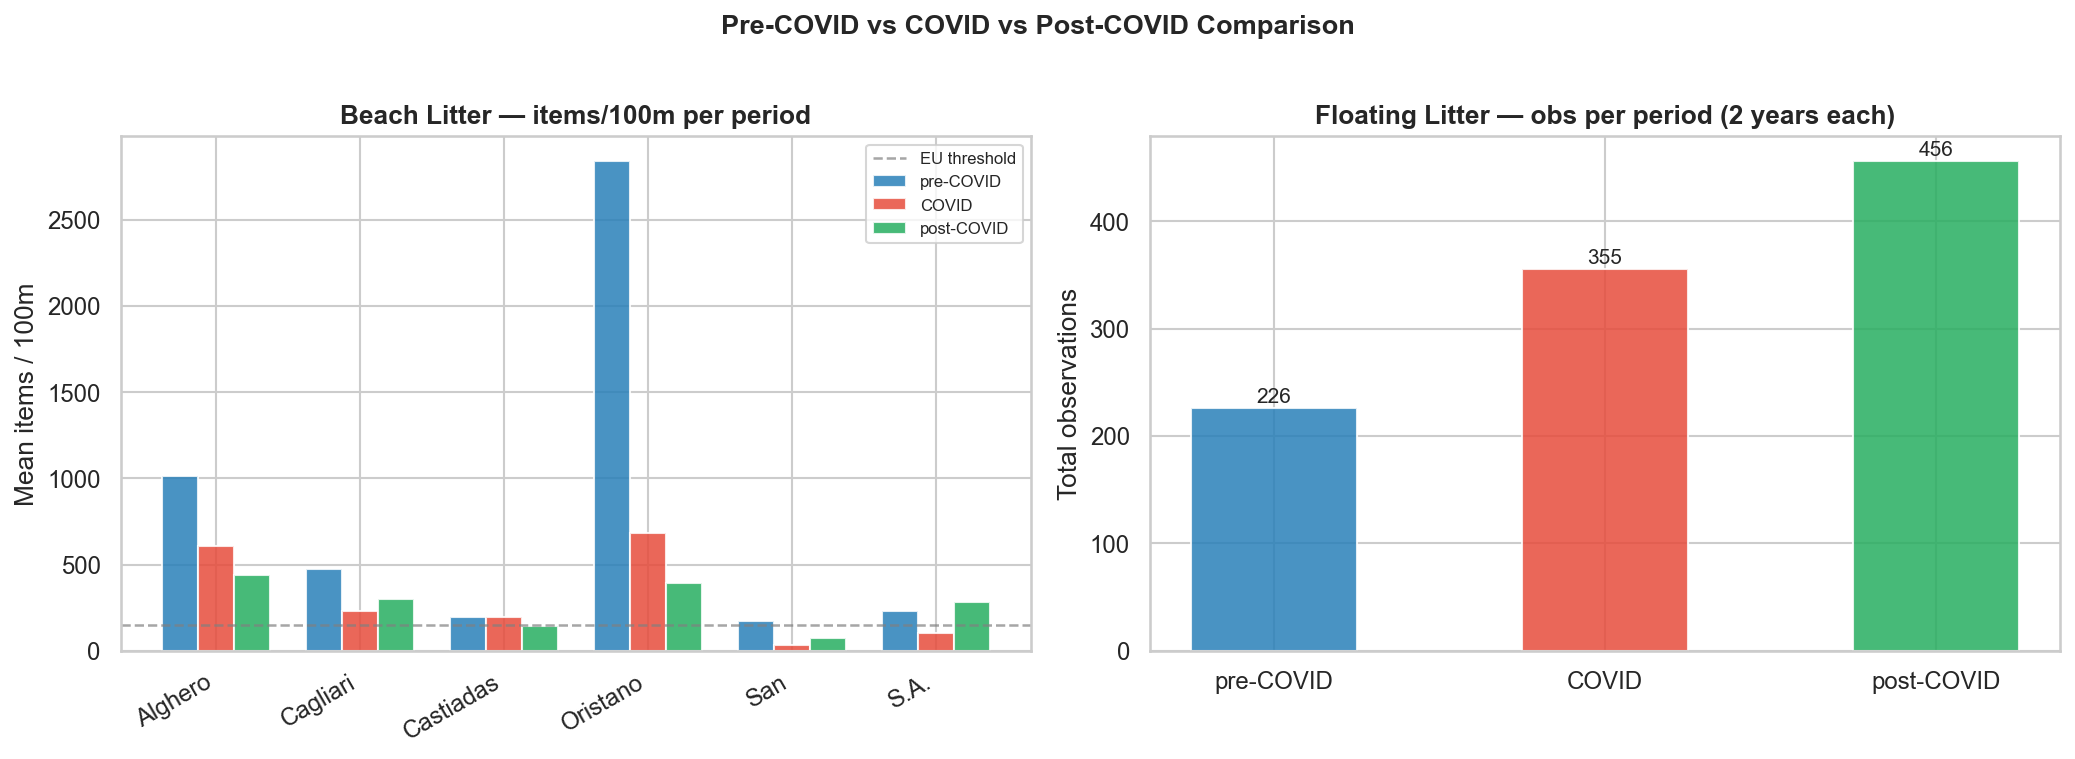
\includegraphics[width=\linewidth]{covid_comparison.png}
\caption{Pre/during/post-COVID comparison.}\end{subfigure}
\caption{Temporal and COVID-period behaviour of beach and floating litter.}
\end{figure}

\end{document}
